\documentclass[sigconf]{acmart}
\settopmatter{printacmref=false} % Removes citation information below abstract
\renewcommand\footnotetextcopyrightpermission[1]{} % removes footnote with conference information in first column
\pagestyle{plain} % removes running headers
\makeatletter
\renewcommand\@formatdoi[1]{\ignorespaces}
\makeatother
\acmDOI{}
\usepackage{amsmath}
\usepackage[ruled,vlined]{algorithm2e}
\usepackage[noend]{algpseudocode}

\settopmatter{printacmref=false} % Removes citation information below abstract
\renewcommand\footnotetextcopyrightpermission[1]{} % removes footnote with conference information in first column
\pagestyle{plain} % removes running headers
%%
%% \BibTeX command to typeset BibTeX logo in the docs
\AtBeginDocument{%
  \providecommand\BibTeX{{%
    \normalfont B\kern-0.5em{\scshape i\kern-0.25em b}\kern-0.8em\TeX}}}


\setcopyright{none}
\begin{document}

\title{Cloud Databases - Final Project Report}

\author{Sebastian Oßner}
\affiliation{%
  \institution{Technical University Munich}
  \city{Munich}
  \country{Germany}}
\email{ossner@in.tum.de}

\author{Calin Buzetelu}
\affiliation{%
  \institution{Technical University Munich}
  \city{Munich}
  \country{Germany}}
\email{ge72xix@mytum.de}

\author{Daniel Krüger}
\affiliation{%
  \institution{Technical University Munich}
  \city{Munich}
  \country{Germany}}
\email{kruegeda@in.tum.de}

\begin{abstract}
  In 2012, Amazon Web Services debuted DynamoDB, a NoSQL storage service that aimed to improve the flexibility and scalability of the traditional relational databases. In the following, we describe our attempt at constructing a storage service with similar goals at heart. This effort was guided along by our instructors during the semester with the workload being broken up into multiple milestones. The most important architectural characteristics, as well as metrics of the final application, will be laid out in the course of this report.
\end{abstract}

\keywords{Cloud Computing, Cloud Databases, NoSQL}

\maketitle
\pagestyle{plain}
\section{Introduction}
% If you looked in the latex file to check why the introduction is so poorly formatted, read the first letter of every line in the introduction pdf :)
Nowadays, AWS advertises DynamoDB first and foremost for its enormous scalability and robustness.
These are the key features viable storage systems provide and features we were tasked with employing in our own database service during the semester. \\Realistically, scalability means not only should our service handle growing loads on single servers, but algorithmic scalability as well. Once the number of storage nodes is scaled up, the overall stability nodes provide should improve.

Noting this as the prime objective, it becomes imperative to use a distributed system of storage nodes that balance the data clients get to the service.

In addition to these main principles, more specifications were gi- ven to us during the semester; As scalability alone is not enough, emulating a feasible storage system would require some redundanc- y and replication mechanisms. A more comprehensive description of our implementations of these requirements is in section \ref{architecture-overview}.

Ultimately, performance will be paramount to providing the utmost throughput to clients. In section \ref{performance-analysis} we provide an in-depth performance analysis of our service.

\begin{center}
  \begin{figure}[htbp]
    \centerline{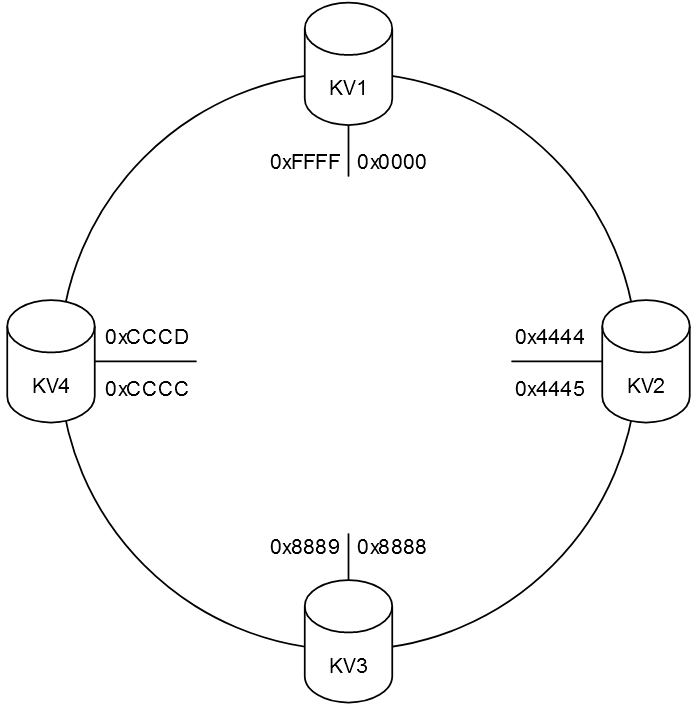
\includegraphics[scale=0.3]{attachments/hashring.png}}
    \caption{A simplified and idealized example of the hashring data structure. In this example, the address of KV2 is hashed to 0x4444, and the address of KV1 to 0xFFFF, which means KV2 is responsible for the range 0x0000-0x4444.}
    \label{fig00}
  \end{figure}
\end{center}

\section{Architecture}\label{architecture-overview}
This section will give a brief overview of the architecture of the main components of our system, these components have mainly been introduced in the later milestones of the course and have proven to show some interesting characteristics. Going forward it is assumed the reader understands the principles behind consistent hashing exemplified by systems such as Apache's "Cassandra".
\subsection{Hashring}
In order to organize the nodes in our storage system, they should be arranged in the form of a hashring.
To do this, the address of every server is hashed using the MD5 algorithm, and the nodes are arranged along the spectrum of possible hash values.

This has the effect that every node can now be assigned a range (e.g. hash of predecessor+1 to hash of the node). Every server in the system has complete information about these ranges. If we were now to insert a key into the storage system and hash the key using MD5, we can assign this key to the server responsible for the range the key is in. An example of this structure can be found in figure \ref{fig00}. If a client is connected to the KVServer that is not responsible for the key, the server provides the client with a metadata update so it can connect to the correct server.

Thanks to this, we can achieve ideal load balancing, as keys are (theoretically) hashed to every server with the same probability.

\subsection{External Configuration Service}
Since the storage nodes in our system are inherently independent of each other, an external service is needed to keep track of them. This external configuration service (ECS) is the coordinator between all the nodes in the system, continuously monitoring servers, keeping track of failures, and relaying information between them.

\begin{center}
  \begin{figure}[htbp]
    \centerline{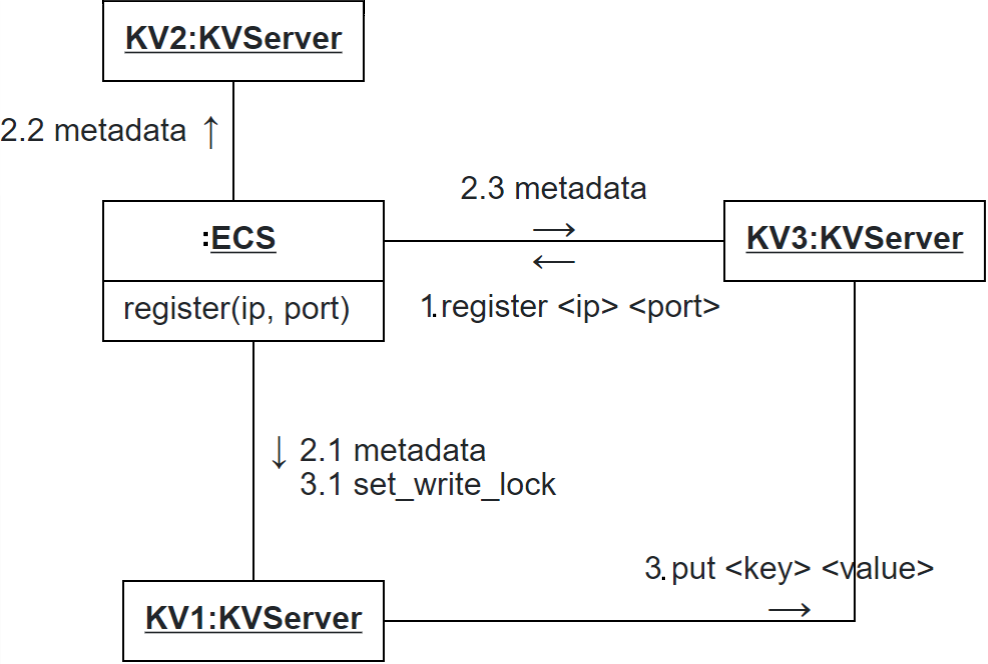
\includegraphics[scale=0.3]{attachments/registration.png}}
    \caption{A simplified communication diagram showing the registration process of a storage node. In this case KV3 is the added server and KV1 is its successor in the hashring.}
    \label{fig01}
  \end{figure}
\end{center}

\subsubsection{Continuous Monitoring}\label{continuous-monitoring}
In order to ensure that the hashring is always up to date, the ECS monitors the servers via pings. The monitoring strategy we chose was heart beating, this is because of its very simple and error-resistant implementation. Heartbeat also makes sense due to the continuous connection our ECS has to the KVServers and the fact that the storage nodes can at times be under heavy load, which is why it is unwise to implement more complex monitoring that would impose an overhead on the nodes.

If a server takes too long to respond, or no message can be sent, the server is considered lost as well as all keys the node stored. In this case, the ECS removes it from its list of active servers, after which the news of the failure needs to be propagated to the other nodes via a metadata update in order to keep the integrity of the hashring.

\subsubsection{Addition and Removal of Storage Nodes}
When a new node starts, it is given the address of the ECS as a bootstrap server and before it can start accepting client connections, it has to register itself at the ECS (see figure \ref{fig01} for a visualization of this process). This is done by establishing a TCP-connection with the bootstrap and sending the register command.
If no reply is received, the node will shut down automatically.

If a server successfully registers, the ECS will notify all other servers of the addition by sending a metadata update consisting of the new hashring.
Then, to initiate the key transfer, the new node's successor is set to read-only and receives the address and port of the new server so it can send the keys which it is no longer responsible for to the new node.

Conversely, if a server wants to deregister because it is being shut down, the server has to send a de-register message to the ECS, after which the ECS manages the rebalancing of keys (analogous to the addition of a node).

\begin{center}
  \begin{figure}[htbp]
    \centerline{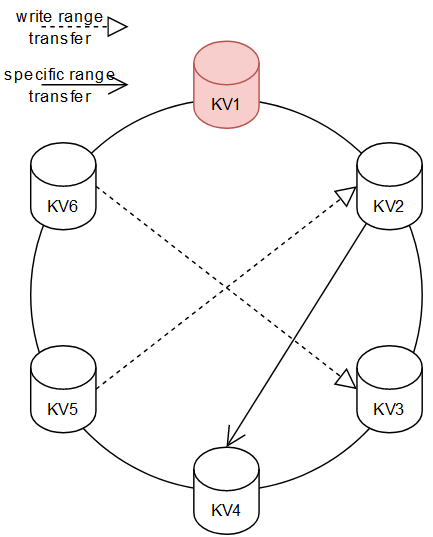
\includegraphics[scale=0.4]{attachments/shutdown_transfer.png}}
    \caption{Example of the transfers necessary to maintain replication balance when a server shutdown is detected. KV1 has been removed from the ring, but the remaining servers need to distribute KV1's responsibilities.}
    \label{fig02}
  \end{figure}
\end{center}


\subsection{Data Replication}
As alluded to in \ref{continuous-monitoring}, if a server can not be reached or does not respond to pings, the keys in this server are considered lost. This of course is understandably undesirable. To ensure that keys are not entirely lost if a server crashes, we now introduce the concept of replication to our storage system.

Replication is achieved by propagating copies of every write request a server receives to its two successors (replicators). These replicators hold copies of the keys and can serve read requests to clients. This is an added bonus, as we thereby decrease the load on the coordination server.

However, this adds a layer of complexity to the additions and removals of nodes to the system. Whereas we previously only concerned ourselves with the split and merge of responsibility ranges, it is now necessary to ensure the integrity of the replication system after changes are made to the structure of the hashring. To achieve this with the minimum number of redundant operations, our team came up with the algorithm shown in \ref{fig02}.

Here, an exemplary server was shut down and removed from the service. However, this node acted as a replicator to its two predecessors, meaning these nodes have to send the keys they are responsible for to their new second successor. The dashed arrows represent a transfer of keys from one server to another where the origin server sends only the keys it has write access to. The solid arrow represents a transfer of keys in an even more specific range, as KV2 now has write access to the keys formerly belonging to KV1, these need to be sent to the second replicator of KV2.

This abstraction is true regardless of the number of nodes in the system. The nodes themselves calculate which server was removed and what their relation to it was.

The rebalancing in the case of a node-addition is much more simple, as it is only necessary that the new server's predecessors send the keys they are responsible for. This would be sufficient for keeping the balance of keys. However, to decrease storage load and prevent stale data from being propagated throughout the system, we decided to also delete the keys servers no longer need to replicate.

\begin{center}
  \begin{figure*}[htbp]
    \centerline{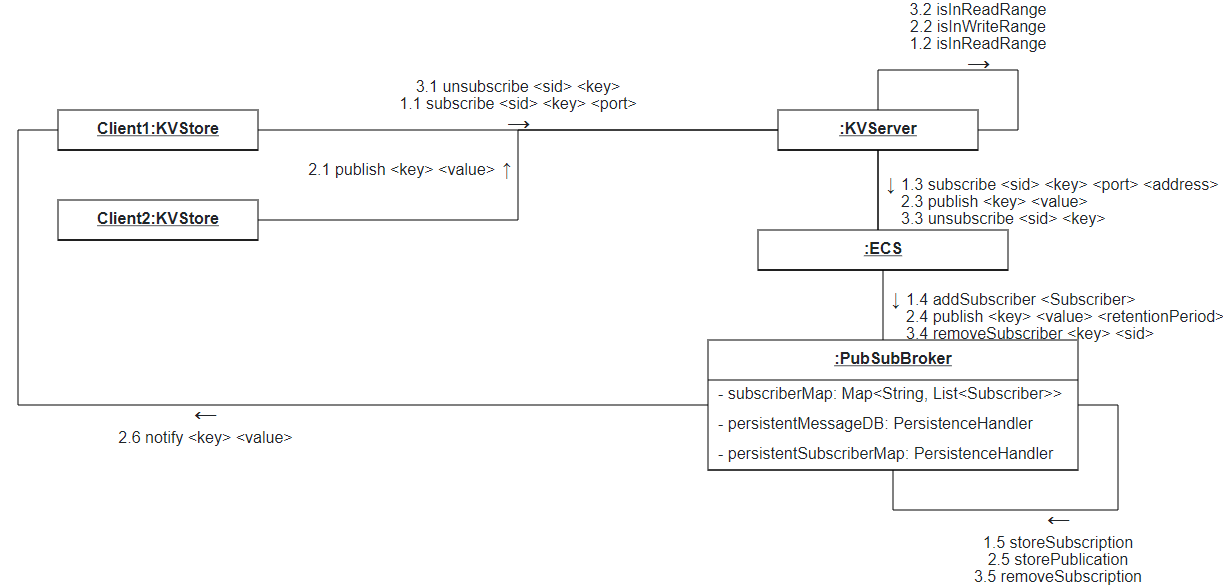
\includegraphics[scale=0.475]{attachments/PubSub.png}}
    \caption{Communication diagram depicting a typical publish/subscribe situation with two individual clients. Here Client1 is a subscriber and Client2 a publisher; After getting notified Client1 unsubscribes from the topic.}
    \label{fig03}
  \end{figure*}
\end{center}

\subsection{Publish/Subscribe System}
In the last iteration of the project, we were tasked with implementing a Publish and Subscribe system (PubSub). With this system, a client can request to be notified whenever a specific key is changed. Per specification and standard, the implementation of this system must exhibit logical decoupling of subscribers and publishers on multiple layers.

The PubSub functionality offers users the possibility of subscribing to some topic of interest, while also receiving a notification for every change incurred on said topic. Any client can subscribe to, or unsubscribe from a topic if the current server he is connected to is either a coordinator or replicator for his key of interest. On the other hand, publication requests can only be sent to the coordinator server of a key. Once the request passes this condition, it is further sent to the ECS, where is processed by the broker. Based on the request type, we store some relevant information not only in a local variable but also in persistent files. We will explain the reasoning behind this system characteristic at a later point in our paper. In the case of a “publish” command, we initiate a non-blocking process for the notification of the subscribed clients. Through the usage of the retention period, the system tries to notify every subscriber of the new value, until said period is reached.
You can observe the communication flow for all the request types offered by the publish-subscribe system in figure \ref{fig03}.

Upon tackling the problem of implementing the publish-subscribe functionality, we realized we have two options, namely, either implement one publish-subscribe broker for every key-value server or implement a centralized broker at the external configuration service side. Our implementation has the broker for the publish-subscribe functionality at the ECS side. We will argue in the following this decision through the lens of a few aspects.

The major argument for choosing this system design is the issue of load-balancing. Assuming our system has a high traffic load with a constant up- and downscale of KVServers, placing an additional broker for the publish-subscribe functionality in the KVServers would prove to add to the aforementioned traffic load.
For every new addition or removal of a KVServer, a transfer to another server of, not only the key-value pairs but also of the subscriptions of the clients would be necessary. Again, assuming our service has a constant high traffic load, this process would prove “exhausting” for the servers and could lead to higher error rates, or even complete server failures. On the other hand, during this time the ECS only deals with the balancing of the server ring in case of a new addition or removal, and the constant monitoring of the servers. With this in mind, we can argue that implementing the publish-subscribe at the ECS side would be beneficial for both the health of the system, as well as the reduction of the failure rate.

\subsubsection{Fault Tolerance}
In our opinion, this problem was one of the most important. We asked ourselves: what is the most important aspect in a system, besides performance and functionality? Thinking of systems we already know about, such as Amazon Web Services, we know that they are highly available, providing clients with their needed functionality day and night. Of course, nothing is 100\% reliable, but, through this system characteristic, we wanted to provide our clients with a high and quick recovery rate of the system, in case of failures. In the broker, additionally to the topic-subscribers map variable that keeps an up-to-date record of the current subscription status, the system also persists all of this information on disk. Due to the possible failure of the system at any time during runtime, this additional feature would allow the service to recover its last “known” state of the subscriptions and resume its functionality as usual. 

Consequently to a possible system (ECS) failure, another problem arose, and namely the recovery of messages which have been lost during their retention period, when the system failed. We tackled this problem in the same way we did for the subscription list. For every “publish” message we receive from a KVServer, that hasn’t had its retention period reached, we persistently store it on disk for recovery, in case of failure. Once the retention period has been reached, we remove it from disk, as any client that hasn’t been online during said period, will not receive a notification message either way. In case of failure, assuming the state of our service remains the same with regards to the number of KVServers and connected clients, the KVServers will automatically try to reconnect to the ECS. Subsequently, the ECS will rebuild its subscriber map from the persistent storage and notify the clients with the messages that haven’t reached their retention period when the ECS had previously failed.

\subsubsection{Delivery Guarantees}
Another important characteristic of a highly available and functioning message-based distributed system is the delivery guarantee. We have approached this trait as an imperative aspect that our system has to ensure. The notification system achieves this through a separate thread, which notifies all clients when a new matching publication for their subscription occurs. The guaranteed delivery is achieved through a confirmation sent from the client, as soon as he receives the notification from the publish-subscribe broker. In case the confirmation isn’t received we know that either the client isn’t connected to the service, or the confirmation has been lost on the way. Consequently, the running notification thread will periodically (every second) retry notifying the clients until we reach the retention period of the message, after which we delete it. In order to ensure a single notification, instead of double, we remove the clients, that we have already notified, from the notification list, based on the receipt of the confirmation message.

\section{Performance Analysis}\label{performance-analysis}
This section concerns itself with the performance of the system. Performance tests will be described in subsection \ref{test-setup}, followed by our expectations and interpretation of the measured values.

\subsection{Test Setup}\label{test-setup}
We split our performance tests into two operation categories - Storage operations and Pubsub operations - and tested them separately.

Storage operations include writing (put, delete) and reading (get) key-value pairs(KV-pairs)  from the storage service. To analyze the difference in performance depending on certain environment configurations, we executed these tests in multiple runs. Our most important factor was scaling. We performed storage operations with an increasing number of storage nodes in each run. We also reran the tests with different cache sizes and cache strategies (First-in-first-out, least-recently-used, least-frequently-used). In each iteration, 1000 different key-value pairs were inserted and accessed, 100 of which were subsequently deleted. We decided to rerun certain tests accessing KVs randomly or frequently to check whether they would be influenced by the caching strategies.
The datasets used for storage operations were KV-pairs of random integers and a set of emails gathered by Enron management. We used random integers mainly to arbitrarily generate any data size we needed for testing. The Enron data set primarily served as a simulation of real-world data. Considering all these factors, this brought us to a total of 65 varying test runs.


\begin{center}
  \begin{figure}[htbp]
    \centerline{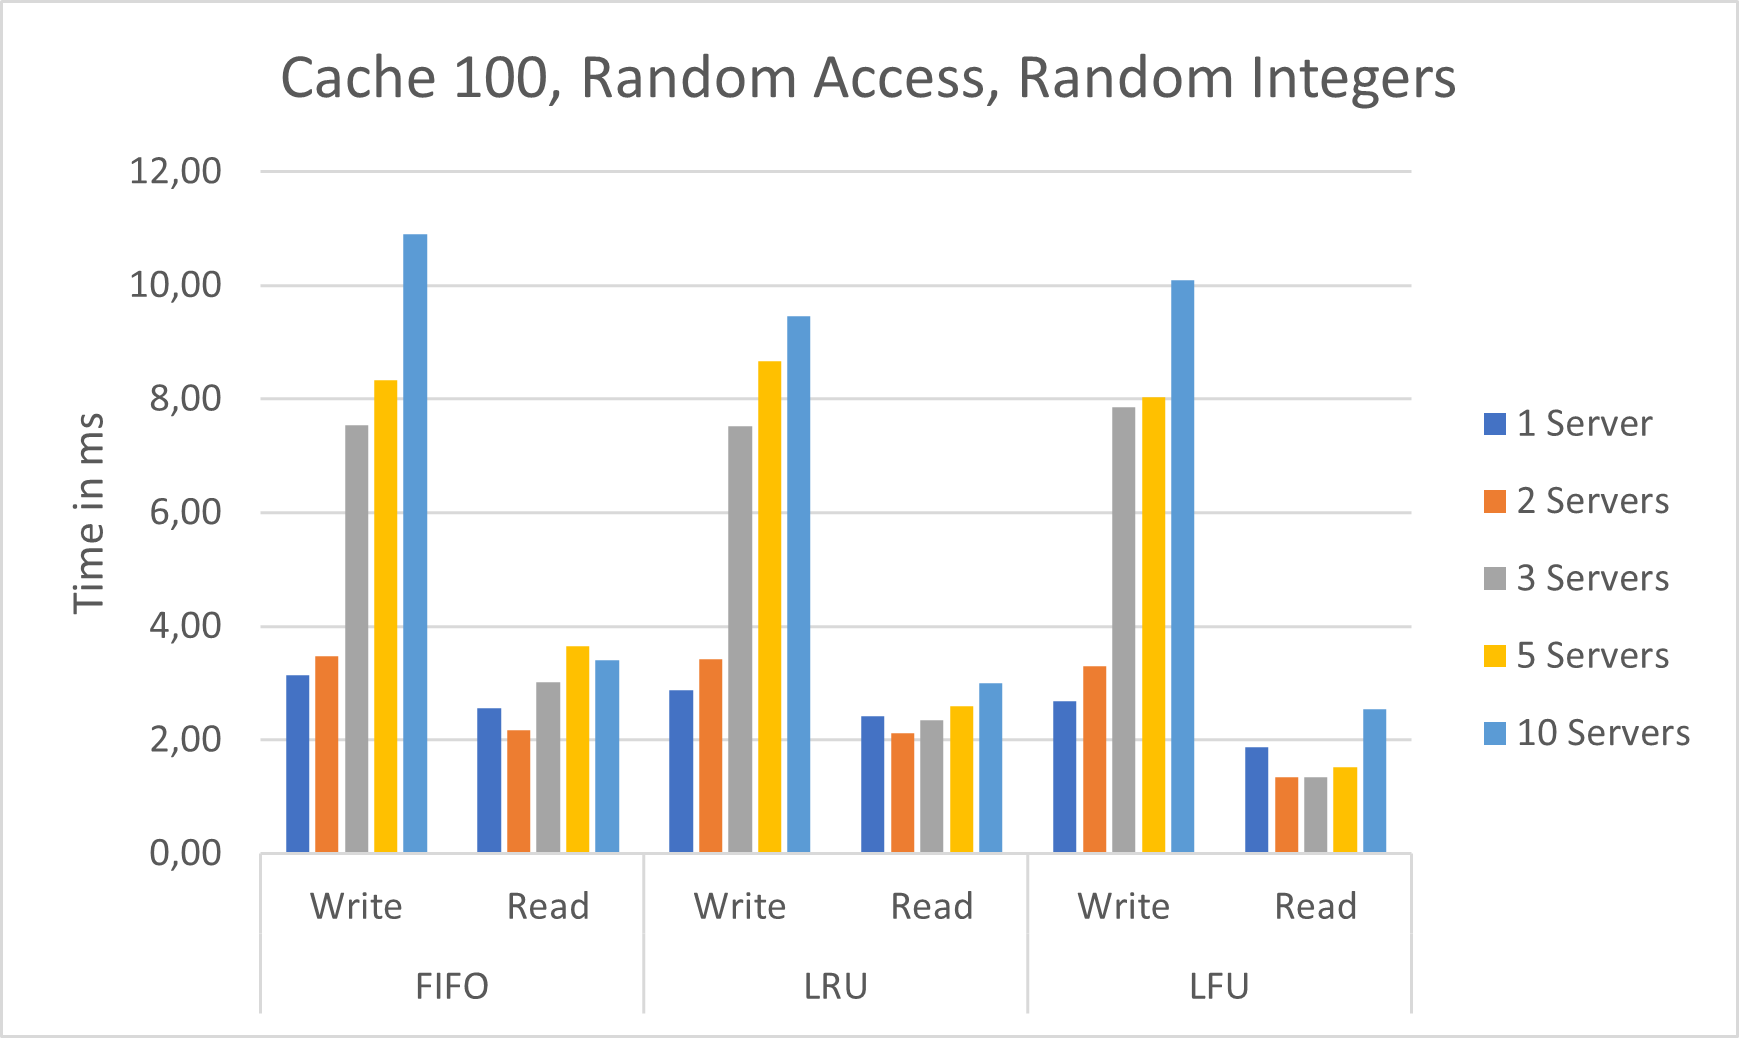
\includegraphics[scale=0.575]{attachments/RandomIntCache100.png}}
    \caption{Bar chart measuring the performance times of 1000 write and read operations under scaling and different strategies with a constant cache size of 100}
    \label{Cache 100}
  \end{figure}
\end{center}



As for the PubSub tests, we were mainly interested in the average time between a publication and notification and the general success rates of a publication. Since PubSub operations are not directly affected by the size of the storage service, we did not require any specific changes to the configuration and therefore only needed few reruns of varying amounts of subscribers. 

\subsection{Expected Results}\label{result-expectation}
We expected the results of storage operations to vary depending on the scale of the storage service, especially when performing get operations. This is mainly due to how replication and the KVserver hashranges depend on the number of running KVservers. A single server may result in fast reads since no reconnections between operations are necessary. However, a server with a large database would slow down performance in case of a cache miss. Two servers would counter this problem, but server connection updates would occur. A ring of three KVServers should deliver the best get times since replication becomes active and each server fully replicates the entire storage database. As a result, no reconnections would be required. On the other hand, write operations should increase significantly, since each inserted/deleted KV would need to be forwarded to all replicating servers. Increasing the scale from this point on could result in longer get times as the hashranges of each KVServer becomes increasingly smaller, making reconnections for each get request more probable.


Additionally, caching should have a major influence on all storage operations. We expect KVServers with small caches to cause frequent cache misses and noticeably increase performance times. When a cache miss occurs, the persistence handler searches through the entire persistent database on disk which is drastically slower than in-memory access. In optimal cases, the KVserver should contain its entire database in cache, however, this may not be feasible in real-world implementations. 

We also suspected that the selected caching strategy would have an effect on performance times. This is because these strategies manage the cache storage and could prevent cache misses depending on the request being handled. If certain KV-pairs were to be requested very frequently, then LRU and LFU would result in a low amount of cache misses. We also believe that FIFO would perform the worst when randomly accessing keys since this strategy is weak against any slight randomness.

\begin{center}
  \begin{figure}[htbp]
    \centerline{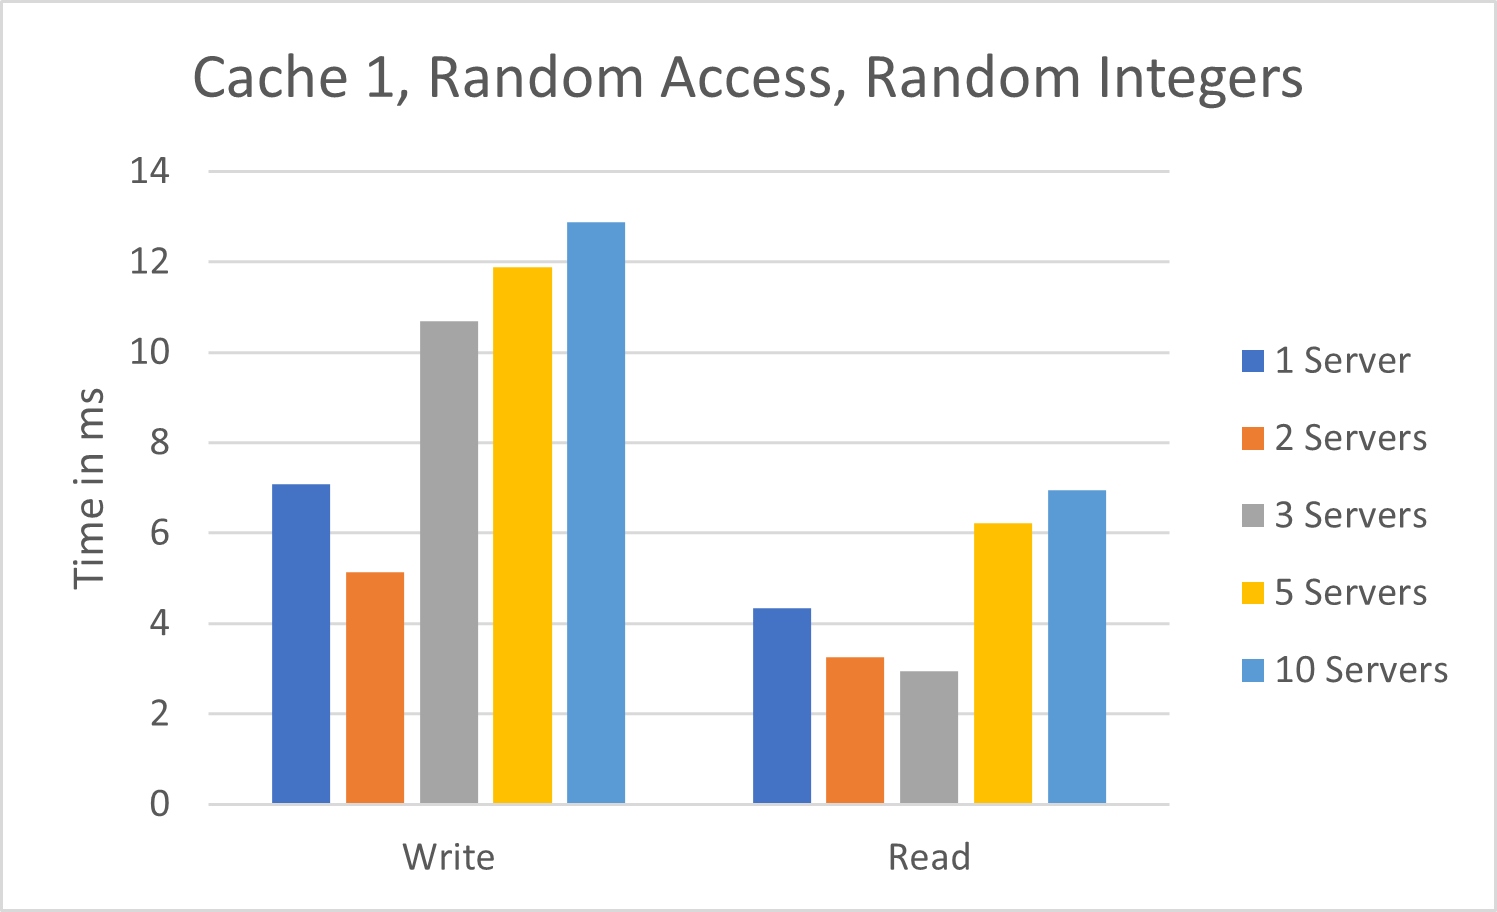
\includegraphics[scale=0.65]{attachments/Cache 1.png}}
    \caption{Performance time measuring operations under scaling with a constant cache size of 1.}
    \label{Cache 1}
  \end{figure}
\end{center}

Finally, the size of KV-pairs could affect multiple factors. First, network transmission of larger messages would lead to longer transport times. Secondly, the server’s storage manager and persistence handler would need to process larger pairs of strings. Therefore, we assume that the Enron data set would perform worse than small KV-pairs such as our random integer data set.

As for our PubSub tests: We were certain that increasing numbers of subscribers would be tightly interrelated to the time between a publication and received notification. Just to be sure that the times were being measured accurately, we also controlled the number of all notifications received.

\subsection{Results and Interpretation}
In figure \ref{Cache 100}, we divert our focus to performance when scaling. A clear trend in performance times when writing can be observed with different numbers of servers. 
It seems that increasing server sizes also led to an increase in time. 
Especially as 3 or more servers were started and replication became active, writing operations latency more than doubled. Since each write operation must also be forwarded to the two replicating servers, extra overhead is added to each request. Furthermore, as the hashring is spread over more and more servers, each server administrates a smaller hashring, making reconnections between each operation more probable. 
As for read operations, we observe that access time performs quite well for storage with less than 10 nodes. Especially 2 servers, since despite reconnecting depending on the key, the chance of receiving from cache is larger than with a single or with multiple servers. 3 Servers also delivers good performance, because no reconnections are required. However, the replicator could deliver a cache miss.

Next, we notice the effect of cache size on writing operations as seen in figure \ref{Cache 1}. A cache size of 1 led to drastically increased latency than tests with larger cache size. The fastest write performance it could deliver for This is due to the server regularly needing to persistently store each request which is in general considerably slower than storing in memory as noted in our expectations.

\begin{center}
  \begin{figure}[htbp]
    \centerline{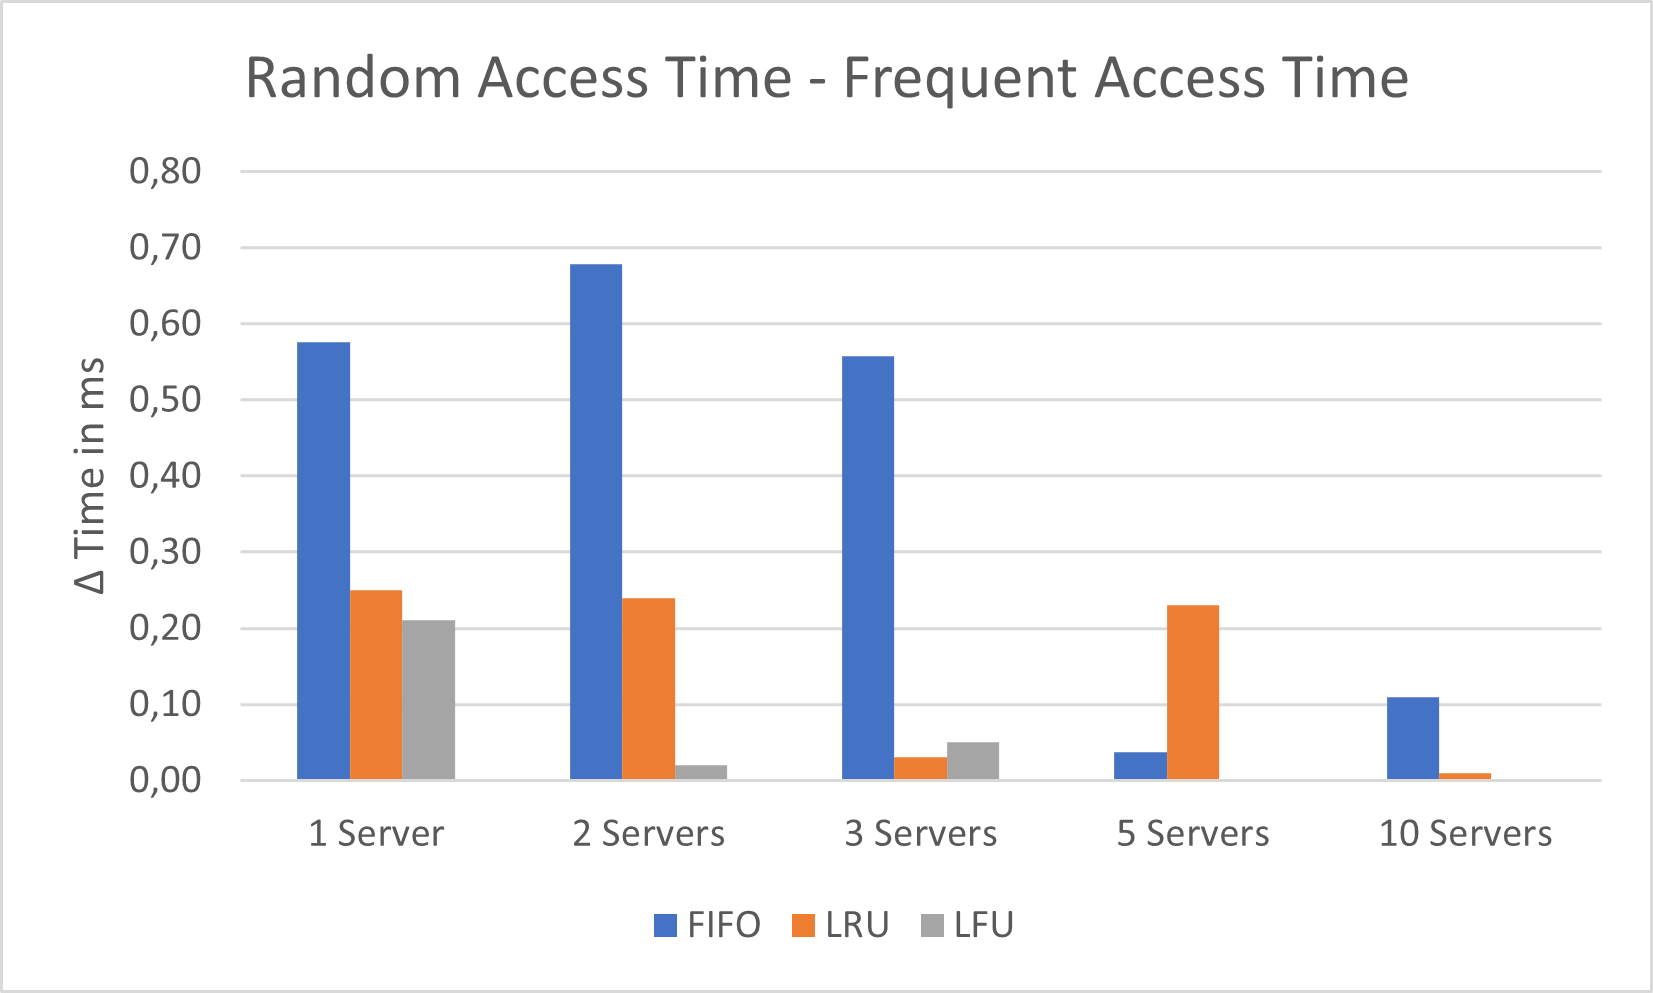
\includegraphics[scale=0.6]{attachments/FrequentAccess.png}}
    \caption{Difference between reading integer pairs when randomly accessing compared to frequently reaccessing certain pairs under scaling and different strategies.}
    \label{FrequentAccess}
  \end{figure}
\end{center}

We were surprised to learn that the caching strategy had very little to no effect when requesting certain keys more frequently. Especially with larger server numbers, the time difference between selecting keys randomly or certain keys more frequently was practically non-existent, as seen in figure \ref{FrequentAccess}. We believe this may be due to the fact that the coordinator and the 2 replicators each manage their own cache. Therefore, even if a client requests a certain key from one server (the key is transferred into cache), when accessing the same key later in time, a connection could be with a different server without this key in cache. To actually make a noticeable difference in performance, the client would have to always connect to the server containing the requested key in cache which would defeat the purpose of offering get ranges. Major contrast was mainly found in the FIFO strategy due to the reduced randomness in our frequent requests test runs.

\begin{center}
  \begin{figure}[htbp]
    \centerline{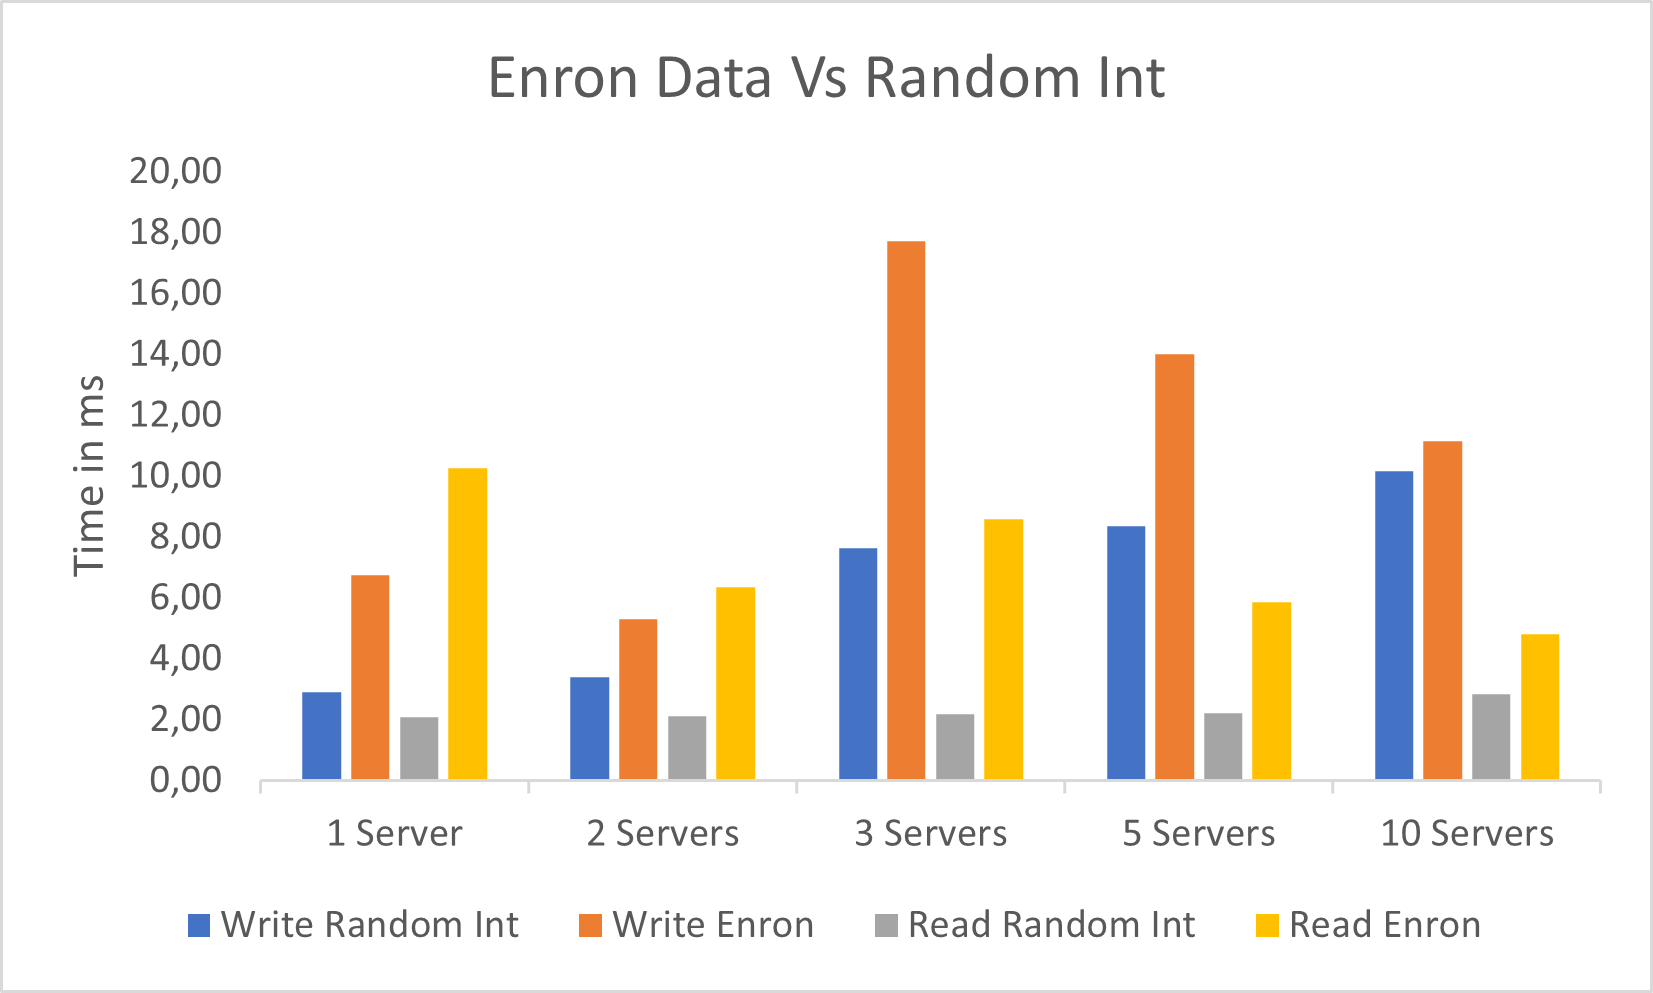
\includegraphics[scale=0.6]{attachments/Enron.png}}
    \caption{Bar chart depicting average operation time using random integer (1000 writes) and Enron data set (400 writes) under scaling. Different strategy times were averaged.}
    \label{Enron}
  \end{figure}
\end{center}

Finally, we analyze the difference in using Enron data in contrast with smaller pairs. As in figure \ref{Enron}, we can see that operations with large KV-pairs like the Enron dataset require much more time than smaller pairs such as random integers. Our explanation in section \ref{result-expectation} seems to suit the results. Important to mention that since we only insert 400 Enron KV-pairs, most of the data is inserted into cache instead of persistency (which was the case with 1000 random integers). Therefore, a decrease in latency can be seen when scaling up. If we were to perform larger bulks of write operations with such a dataset, the write time would rise similarly to the “Write Random Int” bar.

\begin{center}
  \begin{figure}[htbp]
    \centerline{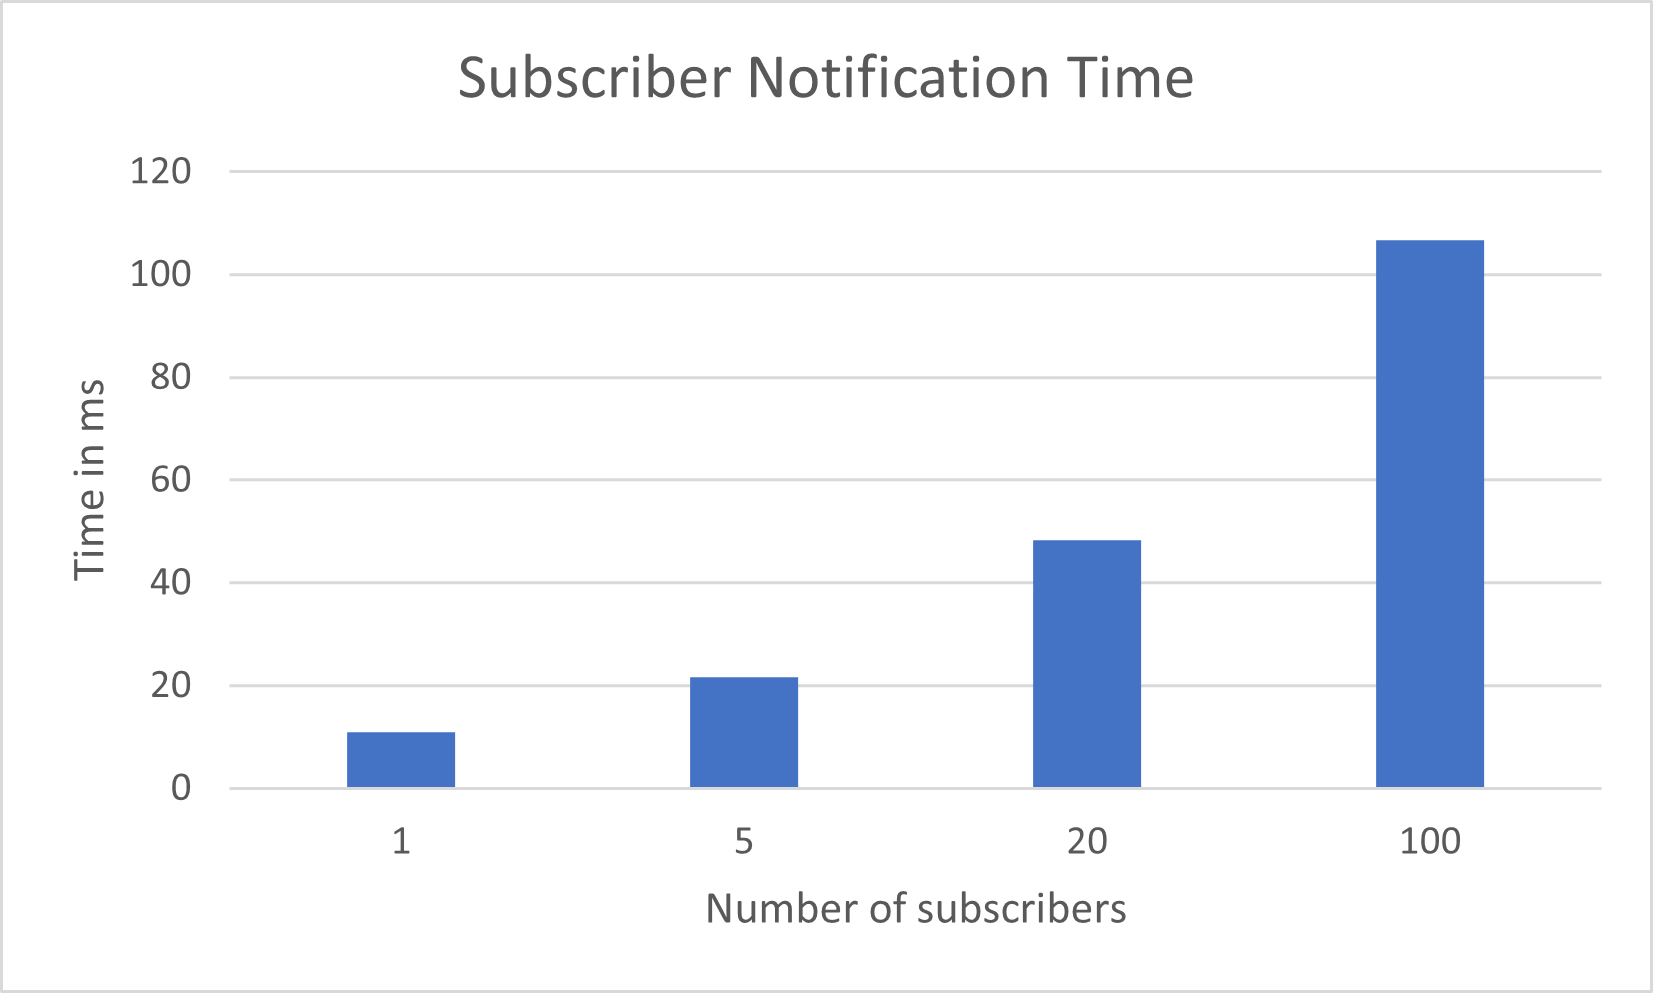
\includegraphics[scale=0.6]{attachments/SubscriberChart.png}}
    \caption{Average time between a publication and notification per subscriber}
    \label{SubscriberChart}
  \end{figure}
\end{center}

As noted in section \ref{result-expectation}, we can clearly see a definite increase. However, we were surprised by the speed of 100 subscribers, since the time-to-subscriber ratio seemed to decrease with larger subscriber numbers. Regrettably, we could not come to a satisfying conclusion as to why this happens. Nevertheless, the time could be affected by the length of the publication message or network latency. The notification success rate was 100\% for all tests which guaranteed that the times were measured accurately. 

\section{Conclusion}
Due to the results gathered in our performance analysis, we conclude that cache sizes have a high influence on the overall performance of the system, as a greater cache decreases costly IO-operations. The choice of cache strategy is also important, as cache misses can be mitigated with more sophisticated strategies.

In optimal cases, the KVserver should contain its entire database in cache, however, this may not be feasible in real-world implementations and could be detrimental in case the server crashed and loses its non-persistent memory. Despite negatively affecting write latency, replication is still recommended to offer raid 1 security. Scaling up should only be performed when replication and load balancing is required. This also offers the benefit of a larger cache. However, the administrator should be wary of the strong relationship between the server address and the hashring to avoid creating an instance with a very small coordination range. Additionally, this will lead to clients reconnecting more frequently to write data.

To bring this report to an end, with the help of instructors, our team has created a scalable and robust storage system while still providing relatively good performance. And although this was our first attempt at creating a cloud storage system (or any cloud application for that matter), we are quite satisfied not only with the final implementation of our assignment but also with the results we have gathered. This course has presented challenging assignments that required hard work and research but also proved to be very rewarding.
\end{document}
\endinput
